\chapter{Software}

\section{Klasse diagram}
Oversigtsklassediagram, se figur \ref{fig:classDiagramSimple}, som fortæller strukturen af namespaces og klasse, men for overskueligheden er alle metoder undladt, se disse under deres respektive afsnit
\begin{figure}[H]
	\includegraphics[width=\textwidth]{Implementeringsdokument/klassediagram_forsimplet-crop.pdf}
	\caption{Forsimplet klasse diagram}\label{fig:classDiagramSimple}
\end{figure}
\newpage

\section{Namespace: GUI Laget}

\begin{figure}[H]
	\includegraphics[width=\textwidth]{klassediagram_GUI-crop.pdf}
	\caption{Klasse diagram over namespacet GUI}\label{fig:classDiagramGUI}
\end{figure}

\subsection{Klasse: Display}
Denne klasse gør brug af to biblioteker for at kunne bruge TFT skærmen, henholdvis Adafruit\_GFX og Adafruit\_ILI9340. For at kunne kommunikere med displayet gøres der brug af disse bibliotekters indbyggede funktioner. Derfor oprettes et objekt af klassen Adafruit\_ILI9340 kaldet TFTscreen.

\subsubsection{Metode: initDisplay()}
\textbf{Parameter: } 
\\ \textbf{Returtype: } \textit{void}
\\ \textbf{Beskrivelse: } Her initieres skærmen med funktion \textit{.begin().} Rotationen og baggrundsfarven af skærmen sættes også når denne metode kaldes. Skærmrotationen er sat 3, hvilket betyder at skærmen er i “landscape mode”. 

\subsubsection{Metode: clearAreaDisp()}
\textbf{Parameter: } \textit{unsigned short pointX, unsigned short pointY, unsigned short width, unsigned short height}
\\ \textbf{Returtype: } \textit{void}
\\ \textbf{Beskrivelse: } Da skærmen baggrundsfarven er sat til sort, medtager denne metode 4 parameter hhv. start x-koordinat, start y-koordinat, bredde og højde. Disse parameter fortæller hvor en del af skærmen der skal farves sort, og dermed slette det område.

\subsubsection{Metode: initConditioning()}
\textbf{Parameter: }
\\ \textbf{Returtype: } \textit{void}
\\ \textbf{Beskrivelse: } Når denne metode kaldes skrives de “faste” værdier på skærmen til et konditioneringsforløb. På billedet nedenfor ses hvordan skærmen ser ud, når metoden er kørt. Et eksempel på hvordan der skrives tekst på skærmen: 
\begin{lstlisting}
TFTscreen.setTextColor(ILI9340_WHITE);  TFTscreen.setTextSize(2);
TFTscreen.setCursor(0, 0);
TFTscreen.println("ID: ");
\end{lstlisting}
Først fortælles hvilken farve teksten skal have, dernæst tekststørrelse og placering. Til sidst angives hvilken tekst der skal printes på skærmen

\begin{figure}[H]
	\includegraphics[width=\textwidth]{billeder/conditioning.png}
	\caption{Layout på displayet når initConditioning() bliver kaldt}\label{pic:conditiong}
\end{figure}

\subsubsection{Metode: initOcclusion()}
\textbf{Parameter: }
\\ \textbf{Returtype: } \textit{void}
\\ \textbf{Beskrivelse: }  Denne metode bruges til at opsætte skærmen for okklusionstræningsforløb. Der skrives tid og enheden for tryk på skærmen. Se billedet nedenfor for layoutet. 

\begin{figure}[H]
	\includegraphics[width=\textwidth]{billeder/occlusion.png}
	\caption{Layout på displayet når initOcclusion() bliver kaldt}\label{pic:occlusion}
\end{figure}

\subsubsection{Metode: initSetup()}
\textbf{Parameter: } 
\\ \textbf{Returtype: } \textit{void}
\\ \textbf{Beskrivelse: } Her opsættes skærmen for setup programmet. Teksten “\textit{Tid pr cyklus}” og “\textit{Antal cyklusser}” er faste værdi på skærmen. Men værdierne hentes fra logik laget, så de er opdateret. 

\begin{figure}[H]
	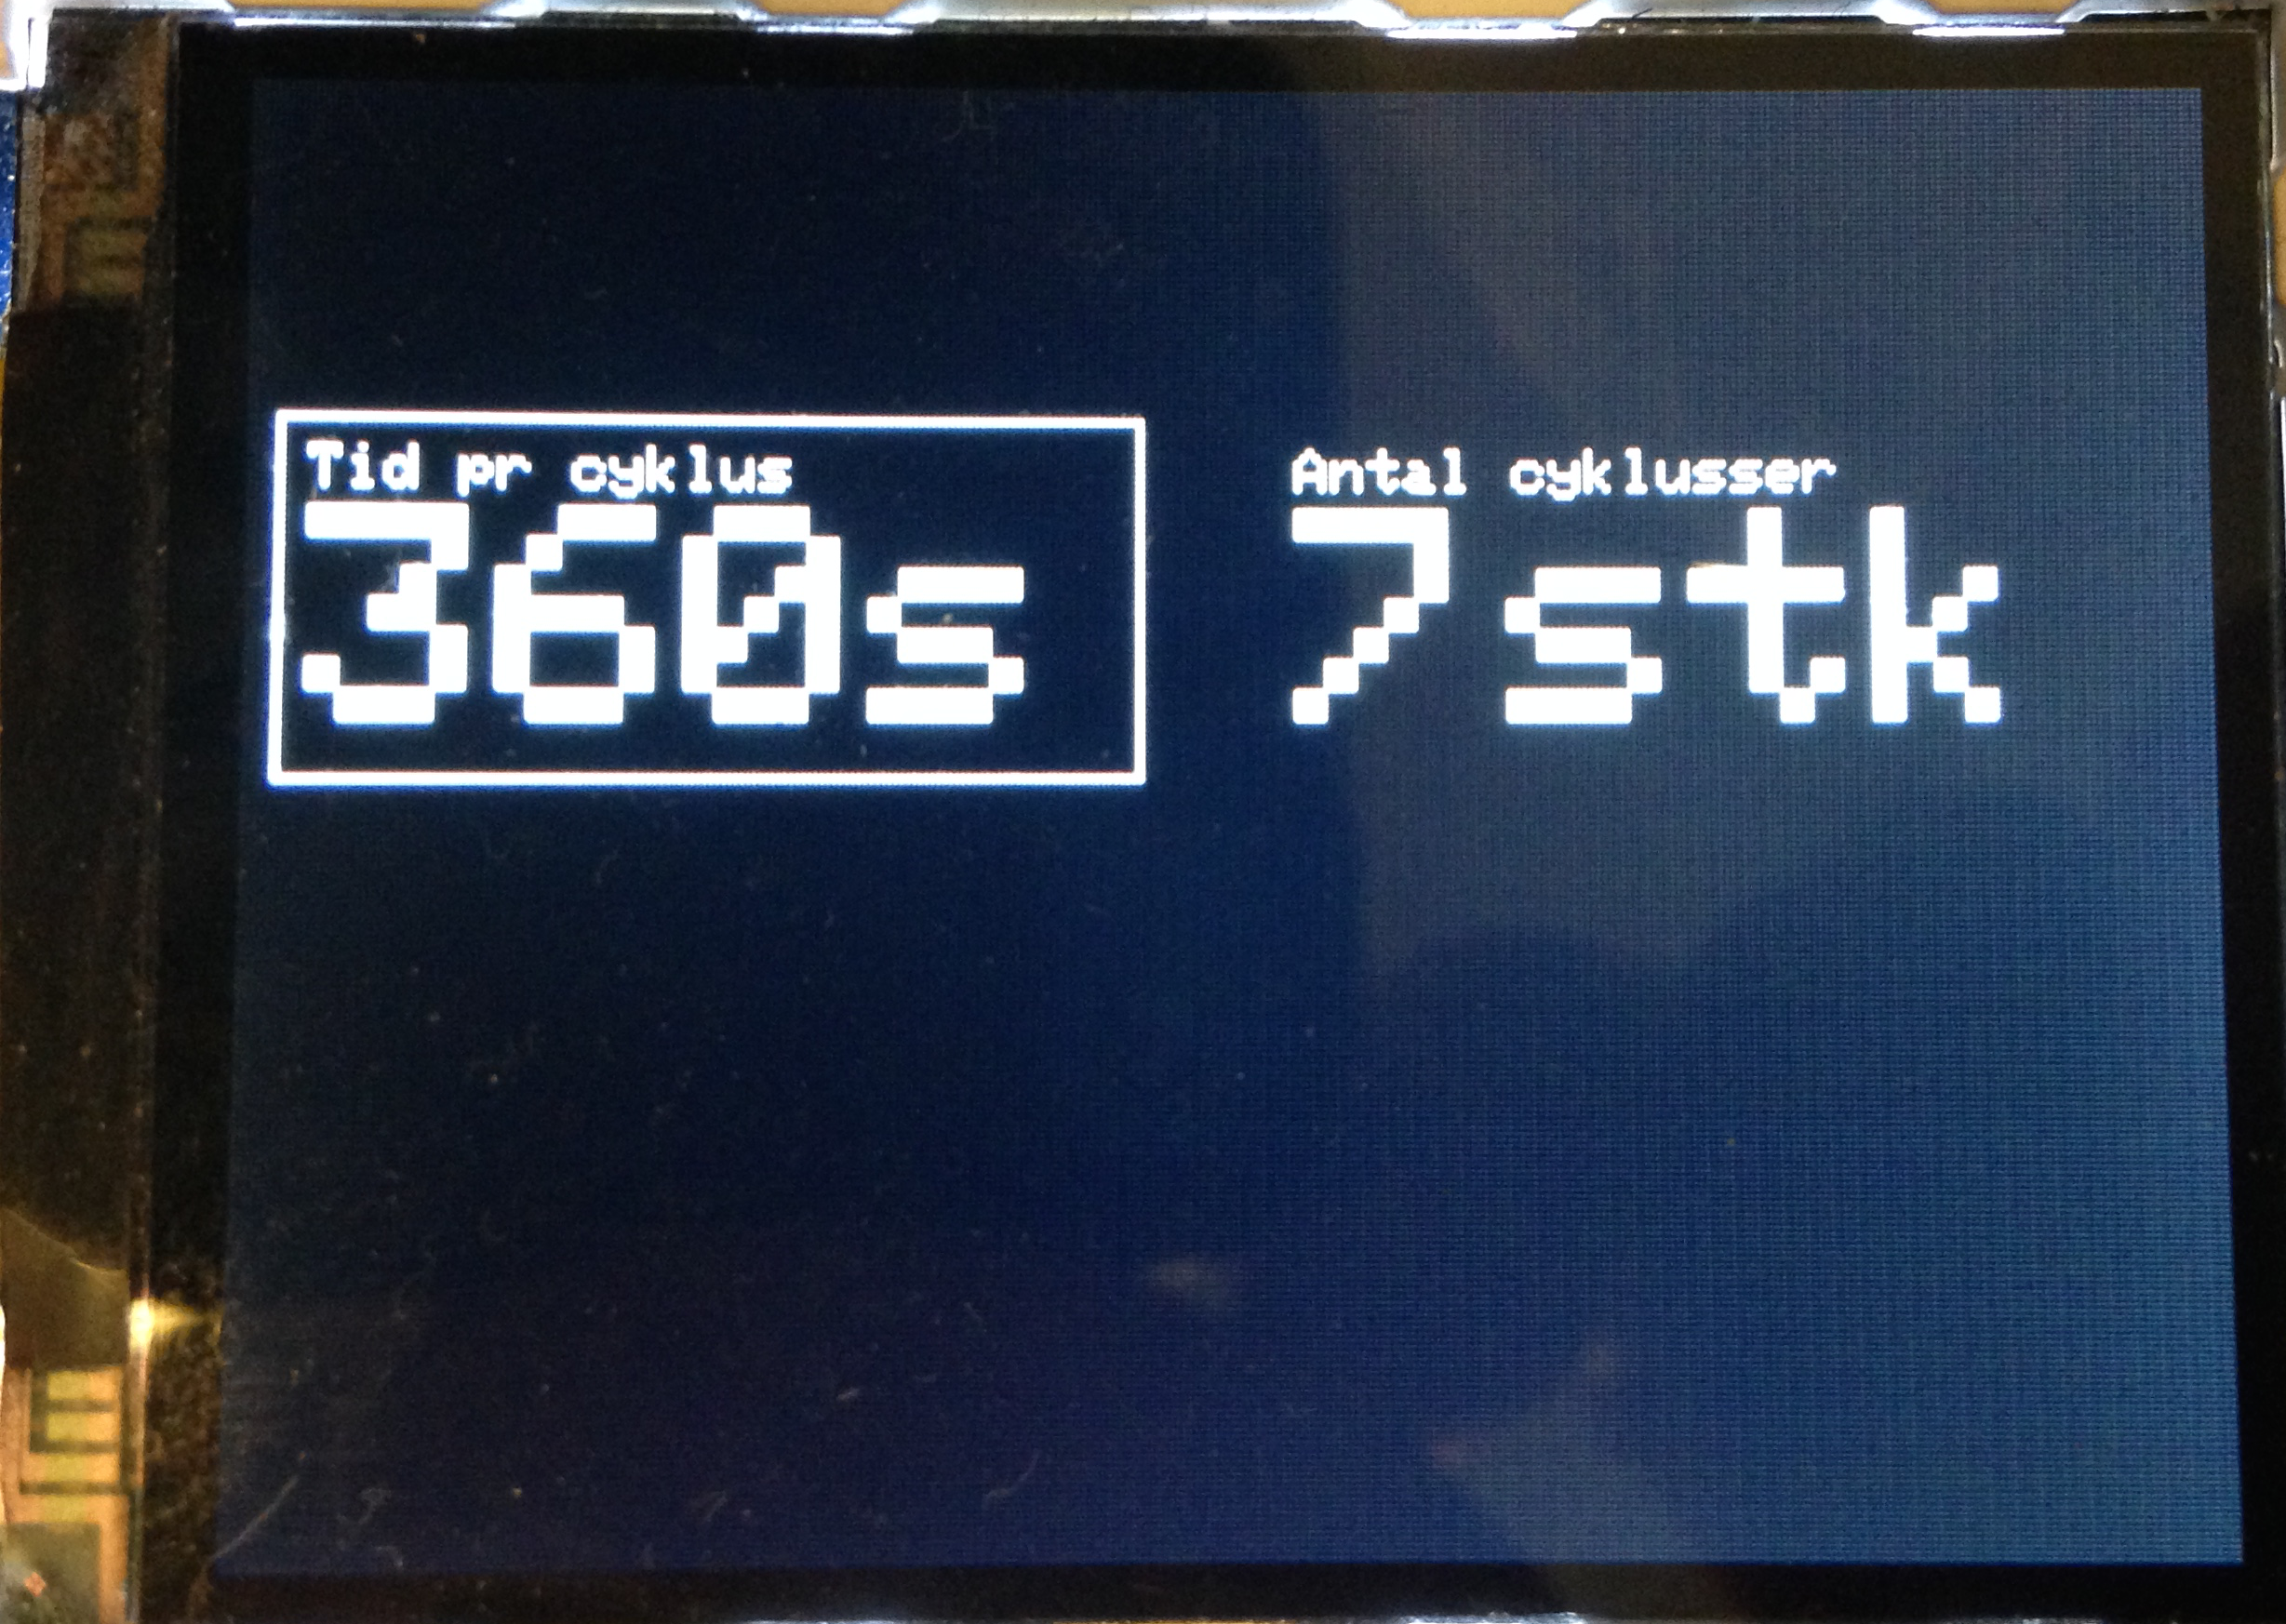
\includegraphics[width=\textwidth]{billeder/setup.png}
	\caption{Layout på displayet når initSetup() bliver kaldt}\label{pic:setup}
\end{figure}

\subsubsection{Metode: moveSquare()}
\textbf{Parameter: } \textit{unsigned short startX, unsigned short startY, unsigned short endX, unsigned short endY, unsigned short width, unsigned short height}
\\ \textbf{Returtype: } \textit{void}
\\ \textbf{Beskrivelse: } Denne metode bruges til at flytte cursoren på skærmen under setup. For at slette noget på skærmen skal det farves samme farve som baggrunden. Derfor får metoden  x- og y-koordinaterne for den firkant der skal slettes, samt x- og y-koordinaterne for hvor den nye firkant skal tegnes henne. Desuden skal metode også have bredde og højde på firkanten. For at sikre at der ikke kan laves et interrupt inde i metode, gør metode brug af den indbyggede funktion \textit{noInterrupt()}. Et interrupt på det forkerte tidspunkt ville betyde at skærm ikke ville slette den forrige firkant eller ikke ville tegne det nye. 

\subsubsection{Metode: updateConditioning()}
\textbf{Parameter: } \textit{volatile bool *buttonPressed, volatile bool *btPressed}
\\ \textbf{Returtype: } \textit{void}
\\ \textbf{Beskrivelse: } Metoden modtager to pointers, som peger på værdien af \textit{buttonPressed} og \textit{btPressen}. Derfor kan metoden i princippet være i 4 forskellige stadier (Se sandhedstabel \ref{tabel:truthtable} )
\begin{table}[H]
	\centering
	\begin{tabular}{|l|l|l|l|l|}
	\hline
	Parameter/Stadie & \textit{Stoppet} & \textit{Konditioneringsforløb} & \textit{Blodtryksmåling} & \textit{Ingenting} \\ \hline
	buttenPressed    & Falsk   & Sand                  & Falsk & Sand            \\ \hline
	btPressed        & Falsk   & Falsk                 & Sand     & Sand        \\ \hline
	\end{tabular}
	\caption{Sandhedstable over \textit{updateConditioning()}s parametre} \label{tabel:truthtable}
\end{table}

Nedenfor er et rammerne for strukturen i metoden, hvor \textit{stadie} stemmer overens med stadierne fra sandhedstabellen. 

\begin{lstlisting}
//***Stadie: Blodtryksmaaling***
if(*btPressed && !*buttonPressed)
{
	//Measure blood pressure and save value to SD card
}
//***Stadie: Konditioneringsforloeb***
if(!*btPressed && *buttonPressed && getNoCycleLeft() != 0)
{
	//Measure blood pressure and save value to SD card
	//Inflate the cuff to systolic pressure + 25mmHg
	
	//Run conditioning in while loop 
}
//***Stadie: Stoppet***
if(!*btPressed && !*buttonPressed){
	//Empty the cuff and clear the sensor value on the dispaly 
	//Reset the number of cycle run in conditioning
}

\end{lstlisting}

Metoden håndtere ikke hvis både \textit{*buttonPressed} og \textit{btPressed} er trykket samtidigt

\textit{buttonPressed} styres ved knaptryk og bruger kan derfor starte og stoppe konditionerings forløbet på denne måde. Hvis forløbet stopper af sig selv, altså hvis antallet af tilbageværende cyklusser er nul, så håndterer metoden at brugeren ikke skal trykke to gange på knappen for at starte et nyt forløb. 
\begin{lstlisting}
	if(memory.getNoOfCycles() == 0)
		*buttonPressed = false;
\end{lstlisting}

\subsubsection{Metode: updateOcclusion()}
\textbf{Parameter: } \textit{volatile bool *buttonPressed}
\\ \textbf{Returtype: } \textit{void}
\\ \textbf{Beskrivelse: } Denne metode køres når apparatet er sat på okklusions træningsforløb. Denne metode bruger også pointeren til \textit{buttonPressed}, hvis den er sand eksekveres et while loop hvor der startes et stopur og trykket fra manchetten vises på skærmen. Hvis værdien er falsk slettes sensorværdien på displayet, og slut tiden vises fra stopuret.

\subsubsection{Metode: updateSetup()}
\textbf{Parameter: } \textit{volatile bool *state}
\\ \textbf{Returtype: } \textit{void}
\\ \textbf{Beskrivelse: } Til styring af cursoren på displayet i setup. Denne metode består af en switch case struktur, som har fire cases og casevalg afgøres af værdien af *state. Case 0 og 1 gør brug af metoden \textit{moveSquare(..)} som flytter cursoren. Case 2 og 3 sørge for at vise værdien af hhv. tid pr cyklus og antal cyklusser. Da cursoren styres med interrupt er interrupts slået fra så længe koden afvikles inde i case 2 og 3. 

\subsubsection{Metode: getNoCycles()}
\textbf{Parameter: } 
\\ \textbf{Returtype: } \textit{unsigned short}
\\ \textbf{Beskrivelse: } Bruges til at hente \textit{antal cyklusser} fra logik laget. Denne værdi aflæses fra EEPROM via data laget, men for at overholde 3-lags modellen skal kommunikation gå via logik laget. 

\subsubsection{Metode: setNoCycles()}
\textbf{Parameter: } \textit{unsigned short value}
\\ \textbf{Returtype: } \textit{void}
\\ \textbf{Beskrivelse: } Bruges til at sætte værdien af \textit{antal cyklusser}. 

\subsubsection{Metode: updateTimeLeft()}
\textbf{Parameter: } \textit{unsigned short value}
\\ \textbf{Returtype: } \textit{void}
\\ \textbf{Beskrivelse: } Denne metode er lavet til opdatere tiden under konditioneringsforløbet. Da det kræver fem kald af metoder fra biblioteket \textit{Adafruit\_ILI9340} for at skrive tekst på skærmen er dette indkapslet i én metode, som blot skal have en String value. Metoden sørge også for at tiden kun opdateres når sekund tælleren på uret ændres

\subsubsection{Metode: updateNoOfCycles()}
\textbf{Parameter: } \textit{String value}
\\ \textbf{Returtype: } \textit{void}
\\ \textbf{Beskrivelse: } Når metoden kaldes opdateres antallet cyklusser på skærmen. Da værdien som metoden modtager indeholder to gange så mange cyklusser som der skal foretages, håndtere metoder at der kun hvis det eksakte antal. Grunden til at der regnes med to gange så mange cyklusser skyldes at programmet intern skal håndtere en okklusion fase og en reperfusions fase for hver cyklus. Håndtering foregår på følgende måde: 

\begin{lstlisting}
	if(value%2)
	valToDisplay = (valToDisplay+1)/2;
	else
	valToDisplay = valToDisplay/2;
\end{lstlisting}

\subsubsection{Metode: updateStopWatchTime()}
\textbf{Parameter: } \textit{unsigned short minutes, unsigned short seconds}
\\ \textbf{Returtype: } \textit{void}
\\ \textbf{Beskrivelse: } Denne metode opdatere tiden fra stopuret på displayet under okklusions træningsforløbet. Displayet opdateres kun når antallet af sekunder på stopuret ændres. 

\subsubsection{Metode: updateBloodPressure}
\textbf{Parameter: } \textit{unsigned short sys, unsigned short dia, unsigned short map)} 
\\ \textbf{Returtype: } \textit{void}
\\ \textbf{Beskrivelse: } Metoden modtager tre parameter med systolisk, diastolisk og middel arterie trykket. Disse værdi konverteres til en String og skrives på skærmen i følgende format: \textit{"120/80(93)"}

\subsection{Klasse: Buttons}

\subsubsection{Metode: readModeSwitch()}
\textbf{Parameter: } 
\\ \textbf{Returtype: } \textit{unsigned short}
\\ \textbf{Beskrivelse: } Denne metode læser to analoge pins hhv; A8 og A9. Her læses stadiet af modeswitch knappen. Hvis A8 er lav(0V) og A9 er høj(5V) køres konditionering, hvis både A8 og A9 er lave køres okklusionstræning og til sidst hvis A8 er høj og A9 er lav køres setup. Denne metode bliver kaldt én gang når arduinoen startes op. Skal der ændres på hvilken forløb apparatet skal køre, skal arduinoen genstartes. 

\subsubsection{Metode: startStopConditioning()}
\textbf{Parameter: } \textit{volatile bool startButtonPressed}
\\ \textbf{Returtype: } \textit{bool}
\\ \textbf{Beskrivelse: } Styring af værdien for \textit{startButtonPressed}. Hver gang metoden køres inverteres værdien af \textit{startButtonPressed}. Desuden indeholder metoden et \textit{if/else} statement, der hvis værdien af \textit{startButtonPressed} er falsk sletter den gamle måling på skærmen og nulstiller antallet af kørte cyklusser. Hvis værdien er sand sættes et tidsstempel, så timeren passer når et nyt forløb startes.  

\subsubsection{Metode: btPressure()}
\textbf{Parameter: } \textit{volatile bool btPressed}
\\ \textbf{Returtype: } \textit{bool}
\\ \textbf{Beskrivelse: } Styring af værdien for \textit{btPressed}. Når denne metode kaldes inverteres værdien af \textit{btPressed}. Hvis værdien er falsk, slettes den sidste måling på skærmen.

\subsubsection{Metode: startStopOcclusion()}
\textbf{Parameter: } \textit{volatile bool startButtonPressed}
\\ \textbf{Returtype: } \textit{void}
\\ \textbf{Beskrivelse: } Her invertes værdien af \textit{startButtonPressed} og returneres. Hvis denne værdi er falsk kaldes en metode fra display klassen som fjerner en værdi på skærmen og der sættes et tidsstempel, fordi at værdien af \textit{startButtonPressed} går fra falsk til sand og derfor skal der startes et okklusionstræningsforløb 

\subsubsection{Metode: changer()}
\textbf{Parameter: } \textit{volatile unsigned short state}
\\ \textbf{Returtype: } \textit{unsigned short}
\\ \textbf{Beskrivelse: } Denne metode bruges til at styre cursoren når der skal ændres i antallet af cyklusser og tiden pr. cyklus. Den modtager værdien state, som kan være et tal mellem nul og tre. Hvis state nul ændres værdien til en og omvendt, det betyder at den skifter mellem at pege på \textit{antal cyklusser} og \textit{tid pr cyklus}. 
Hvis state har værdien to ændres der på \textit{tid pr. cyklus }og hver gang metoden kaldes forøges værdien tid pr. cyklus med 30 sekunder. Desuden håndtere metoden at denne værdi kun kan ændres i intervallet mellem 180 til 480 sekunder, dvs 3 til 5 minutter. Hver gang værdien \textit{tid pr cyklus} ændres, skrives den nye værdi til EEPROM via metoden \textit{InternalMemory::setTimePerCycles()}. 
Når state er lige med 3, ændres værdien af antal cyklusser og denne værdi forøges med 1 cyklus hver gang knappen trykkes. Denne værdien kan ændres i intervallet mellem 1 og 5 cyklusser. Den nye værdi skrives til EEPROM. 

\subsubsection{Metode: selector()}
\textbf{Parameter: } \textit{volatile unsigned short state}
\\ \textbf{Returtype: } \textit{unsigned short}
\\ \textbf{Beskrivelse: } Metoden \textit{selector()} ændres udelukkende på værdi af \textit{state} og returnerer den nye værdi af \textit{state}. 


\section{Namespace: Logik laget}

\begin{figure}[H]
\includegraphics[trim = 0 170 0 0, clip = true, width=\textwidth]{klassediagram_Logic-crop.pdf}
\caption{Klasse diagram over namespacet Logic}\label{fig:classDiagramLogic}
\end{figure}

\subsection{Klasse: BPalgorithm}

\subsubsection{Metode: calculateMap()}
\textbf{Parameter: } \textit{unsigned short peaks[], unsigned short cuffPressure[], unsigned short peakArrayLength, unsigned short *totalNumberOfPeaks}
\\ \textbf{Returtype: } \textit{unsigned short}
\\ \textbf{Beskrivelse: } Denne metode beregner MAP ud fra digitalt filtreret peakdata i peaks[] og cuffPressure[]. MAP findes som trykket i manchetten ved den højeste peak amplitude (se figur \ref{fig:bpMeasurement})

\newpage
\begin{figure}[H]
	\includegraphics[width=\textwidth]{billeder/Alpha015-crop.pdf}
	\caption{Graf med data fra en blodtryksmåling på simulator(120/80)}\label{fig:bpMeasurement}
\end{figure}
Her ses at det rå signal er støjfyldt. Sort er manchet trykket, blå er de rå peak amplituder, rød er filtreret en gang fra venstre mod højre, sort	er filtreret fra begge sider.

\subsubsection{Metode: calculateSYS()}
\textbf{Parameter: } \textit{unsigned short peaks[], unsigned short cuffPressure[],unsigned short peakArrayLength, unsigned short *totalNumberOfPeaks, unsigned short MAP}
\\ \textbf{Returtype: } \textit{unsigned short}
\\ \textbf{Beskrivelse: } Denne metode beregner SYS ud fra MAP og digitalt filtreret peakdata i peaks[] og cuffPressure[]. SYS findes som trykket i manchetten ved peak amplituder på 38\% af MAP. (Se figur \ref{fig:bpMeasurement})

\subsubsection{Metode: calculateDIA()}
\textbf{Parameter: } \textit{unsigned short peaks[], unsigned short cuffPressure[],unsigned short peakArrayLength, unsigned short *totalNumberOfPeaks, unsigned short MAP}
\\ \textbf{Returtype: } \textit{unsigned short}
\\ \textbf{Beskrivelse: } Denne metode beregner DIA ud fra MAP og digitalt filtreret peakdata i peaks[] og cuffPressure[]. DIA findes som trykket i manchetten ved peak amplituder på 48\% af MAP. (Se figur \ref{fig:bpMeasurement})

\subsection{Klasse: DigitalFiltering}

\subsubsection{Metode: averagingZeroGroupDelay()}
\textbf{Parameter: } \textit{nsigned short peaks[],unsigned short peakArrayLength, unsigned short *totalNumberOfPeaks, double alpha}
\\ \textbf{Returtype: } \textit{void}
\\ \textbf{Beskrivelse: } Denne metode anvender eksponentiel midligsfilter teknik (Se afsnit \ref{title:digitalFilter}) uden group delay til at midle over parameteren peaks.
\begin{lstlisting}
	peaks[0] = startValue;
	peaks[totalNOPeaks] = startValue;
	for(i = 1;i<totalNOPeaks; i++)
	{
	peaks[i] = alpha*peaks[i]+(1-alpha)*peaks[i-1];
	}
	
	for(i = totalNOPeaks-1;i>0; i--)
	{
	peaks[i] = alpha*peaks[i]+(1-alpha)*peaks[i+1];
	}
\end{lstlisting}

\subsection{Klasse: Scenarios}

\subsubsection{Metode: bloodPressure()}
\textbf{Parameter: } \textit{unsigned short *MAP, unsigned short *SYS, unsigned short *DIA, BPAlgorithm bpa, Data::PressureControl pc, Data::PressureSampling ps, Logic::DigitalFiltering df, Utilities util}
\\ \textbf{Returtype: } \textit{void}
\\ \textbf{Beskrivelse: } Denne metode indeholder opskriften til en blodtryksmåling. Det vil sige at kaldes metoden, udføres en blodtryksmåling og alle andre klasser og metoder, som skal bruges til dette eksekveres inde i denne metode. Pointerne til de tre variabler får værdierne MAP, SYS og DIA fra blodtryksmålingen.

\subsubsection{Metode: occlusiontraining()}
\textbf{Parameter: } \textit{volatile bool *start}
\textbf{Returtype: } \textit{unsigned }
\textbf{Beskrivelse: } Denne metode metoder en bool værdi, som afgøre hvilke to stadie metoden skal eksekveres i. Hvis \textit{start} er true, lukkes ventil og med en if sætning pumpes manchetten op til mimimum 90 mmHg og hvis trykket overstiger 100 mmHg slukkes motoren. 
Hvis metoden modtager en falsk værdi slukkes motoren og ventilen åbnes. 

\subsubsection{Metode: occlude()}
\textbf{Parameter: } \textit{unsigned short pressure}
\textbf{Returtype: } \textit{unsigned short}\\
\textbf{Beskrivelse: }Metode der bruges i konditioneringsforløbet når blodtrykket er bestemt og der skal laves en afklemning. Først indhentes det nuværende manchet tryk. Dernæst bruges den parameteren \textit{pressure}, som indeholder det systoliske blodtryk, til at bestemme hvor meget manchetten skal fyldes. Der søges for at trykket i manchetten mindst bliver 200mmHg og maks 300mmHg. Efter dette indeholder \textit{pressure}  afklemningstrykket og motoren begynder at pumpe indtil trykket i manchetten er større end \textit{pressure} + 10. Plus 10 fordi at motoren drifter en anelse og ikke stopper præcist ved det tryk der specificeres. 
Hvis metoden modtager 0 istedet for det systoliske tryk, åbnes ventilen og manchetten tømmes indtil trykket er under 10mmHg. 


\subsection{Klasse: Timer}
Klassen timer gør brug af en hardware Real Time Clock(RTC) med IC’en \textit{DS1302}. For at kommunikere med denne RTC, så gør klassen brug af et biblioteket \textit{DS1302}. Derfor oprettes et objekt af klassen \textit{DS1302.h} ved navn timestamp. Et Time objektet indeholder hhv: år, måned, dag, time, minut, sekund og ugedag. 

\subsubsection{Metode: setTimeStamp()}
\textbf{Parameter: } 
\\ \textbf{Returtype: } \textit{void}
\\ \textbf{Beskrivelse: } Denne metode aflæser den nuværende værdi af timeren og sætter en variable til denne værdi. 

\subsubsection{Metode: getTimeStamp()}
\textbf{Parameter: } 
\\ \textbf{Returtype: } \textit{Time}
\\ \textbf{Beskrivelse: } Returnerer et Time objekt med værdien af timestamp. 

\subsubsection{Metode: countdown()}
\textbf{Parameter: } \textit{unsigned short totalTime}
\\ \textbf{Returtype: } \textit{void}
\\ \textbf{Beskrivelse: } Denne metode modtager parameteren \textit{totalTime}, som indeholder det ønskede antal sekunder nedtællingen skal vare. Variablen \textit{elapsedTime} indeholder den nuværende tid og timestamp indeholder et tidsstempel der bliver sat når timeren skal starte. Hver gang metoden køres trækkes den nuværende tid i hhv timer, minutter og sekunder fra hinanden. Dernæst omregnes de forskellige difference til samlede antal sekunder, hvorefter det tal omregnes til sekunder og minutter. For at få antal sekunder tages differencen mellem \textit{totalTime} og \textit{elapsedTotalSeconds} udregner modulus 60 til dette tal(Se formel \ref{eq:totalSeconds})
\begin{equation} \label{eq:totalSeconds}
seconds = (totalTime - elapsedTotalSeconds) \bmod 60
\end{equation}

Dette samme gøres for minutter blot hvor \textit{seconds} også trækkes fra. Se kode nedenfor. 
\begin{lstlisting}
	timerHasEnded = false;
	Time elapsedTime = rtc.time();
	String elapsedTimeString;
	unsigned short hoursToSec = (elapsedTime.hr-timestamp.hr) * 24	* 60;
	unsigned short minutesToSec = (elapsedTime.min- timestamp.min)	* 60;
	unsigned short elapsedTotalSeconds = hoursToSec + minutesToSec	+ (elapsedTime.sec - timestamp.sec);
	seconds = (totalTime - elapsedTotalSeconds) % 60;
	minutes = (totalTime - elapsedTotalSeconds - seconds)/60;
	
	if(minutes == 0 && seconds == 0)
	timerHasEnded = true;
\end{lstlisting}
Når det er regnet ud hvor mange minutter og sekunder der er tilbage i nedtællingen, gemmes de lokale variable minutes og seconds. 

\subsubsection{Metode: stopWatch()}
\textbf{Parameter: } 
\\ \textbf{Returtype: } \textit{void}
\\ \textbf{Beskrivelse: } Metode til at styre simulere og styre et stopur under okklusionstræning, den forløbne tid udregnes på samme måde \textit{countdown()}, blot hvor det er tidsstemplet der trækkes fra den nuværende tid. Denne metode gemmer også minutter og sekunder i to lokale variabler, når udregning er den forløbne tid er færdig. 

\subsubsection{Metode: displayTimer()}
\textbf{Parameter: }
\\ \textbf{Returtype: } \textit{ String}
\\ \textbf{Beskrivelse: } Denne metode bruges til at konvertere tiden fra enten stopuret eller nedtællingen til formatet mm:ss. Desuden konverteres tiden til en string. 
\begin{lstlisting}
	String minString = String(minutes, DEC);
	String secString = String(seconds, DEC);
	String timeString;
	
	if(0 <=minutes && minutes < 10)
	minString = String("0" + minString);
	else
	minString = String(minutes, DEC);
	
	if(0 <=seconds && seconds < 10)
	secString = String("0" + secString);
	else
	secString = String(seconds, DEC);
	return timeString = String(minString + ":" + secString);
\end{lstlisting}
For at sikre at tiden vises på formatet mm:ss, tjekker metoden for om \textit{seconds} eller \textit{minutes} er større eller lig med 0 og mindre end 10. Hvis det er tilfældet tilføjes et nul foran værdien 

\subsubsection{Metode: getTimerStatus()}
\textbf{Parameter: } 
\\ \textbf{Returtype: } \textit{bool}
\\ \textbf{Beskrivelse: } Metode til at returnere værdien af statussen for timeren, hvis værdien er sand er timeren slut og omvendt hvis værdien er falsk kan timeren stadig være igangværende. 

\subsubsection{Metode: setTimerStatus()}
\textbf{Parameter: } \textit{bool val}
\\ \textbf{Returtype: } \textit{void}
\\ \textbf{Beskrivelse: } Denne metode bruges til at sætte værdien af statussen for timeren, den sættes til true for at stoppe timeren. Derfor modtager en metode en parameter af typen bool. 

\subsubsection{Metode: timeToString()}
\textbf{Parameter: } 
\\ \textbf{Returtype: } \textit{String}
\\ \textbf{Beskrivelse: } For at kunne gemme tidsstempler på SD kortet, er denne metode lavet til at konvertere et tidsstempel til en string på formatet: \textit{tt:mm:ss DD-MM-YY}. Ligesom metoden \textit{displayTimer()} håndterer denne metode hvis enten timer, minutter eller sekunder er mindre end 10 og sætter et nul foran. Metoden returnere en samlede string med et tidsstempel 

\subsection{Klasse: MemoryParser}
Denne klasse er lavet for at overholde 3-lags modellen. Da informations læsning fra fx EEPROM og SD kort skal foregå i data laget, skal der en række metoder til at sende information igennem logik laget og videre til GUI laget. Derfor indeholder denne klasse som udgangspunkt kun get og set metoder. 

\subsubsection{Metode: getNoOfCycles()}
\textbf{Parameter: } 
\\ \textbf{Returtype: } \textit{unsigned short}
\\ \textbf{Beskrivelse: } Denne metode returnere værdien fra data laget via metoden \textit{“intMem.readFromEEPROM()”}.

\subsubsection{Metode: setNoOfCycles()}
\textbf{Parameter: } \textit{unsigned short val}
\\ \textbf{Returtype: } \textit{void}
\\ \textbf{Beskrivelse: } Metode der skriver til data laget via metoden: \textit{intMem.writeToEEPROM(200, val)}. Parameteren \textit{val} videres til med denne metode. 

\subsubsection{Metode: getTimePerCycle()}
\textbf{Parameter: } 
\\ \textbf{Returtype: } \textit{unsigned short}
\\ \textbf{Beskrivelse: } Da værdien af timePerCycle indeholder hvor mange sekunder én konditioneringscyklus skal vare, er denne værdi ofte større end 255. Denne værdi skal læses fra EEPROM og en plads kan indeholde værdier på maks 255. Derfor sørger metoden for at hente værdien fra den anden plads, hvis den er større end maks værdien. 
\begin{lstlisting}
	unsigned short val = intMem.readFromEEPROM(205);
	unsigned overloadVal = 0;
	if(val == 255)
	return overloadVal = val + intMem.readFromEEPROM(206);
	else
	return val;
\end{lstlisting}


\subsubsection{Metode: setTimePerCycle()}
\textbf{Parameter: } \textit{unsigned short val}
\\ \textbf{Returtype: } \textit{void}
\\ \textbf{Beskrivelse: } Beskrivelse: Når denne metode køres skrives tiden pr. cyklus til EEPROM, som forklaring i metoden \textit{getTimePerCycle()}, skal den metode håndtere overload. 
\begin{lstlisting}
	if(val > 255){
	unsigned short rest = val % 255;
	unsigned short valtoFit = val - rest;
	intMem.writeToEEPROM(205, valtoFit);
	intMem.writeToEEPROM(206, rest);
	}
	else
	intMem.writeToEEPROM(205, val);
\end{lstlisting}
Det er forinden bestemt at adresserne 205 og 206 bruges til at gemme \textit{TimePerCycle}. Metoden får en parameter som indeholder antallet af sekunder en cyklus skal vare, og for sørge for værdien skrives korrekt til EEPROM udregnes modulus 255 af antallet af sekunder og den rest gemmes på adressen 206. 

String timeStamp, boolean occlusionComplete, unsigned short occlusionPressure, unsigned short sys, unsigned short map, unsigned short dia, boolean interruptOcclusion

\subsubsection{Metode: writeToSDCard()}
\textbf{Parameter: } \textit{String timeStamp, boolean occlusionComplete, unsigned short occlusionPressure, unsigned short sys, unsigned short map, unsigned short dia, boolean interruptOcclusion}
\\ \textbf{Returtype: } \textit{void}
\\ \textbf{Beskrivelse: }  Denne metode indeholder syv parametre af typerne \textit{String}, \textit{boolean} og \textit{unsigned short}. Metoden konverterer og samler alle parametrene til en string og ved denne sendes videre til datalaget.

\subsubsection{Metode: getID()}
\textbf{Parameter: }\textit{}
\textbf{Returtype: } \textit{String}
\textbf{Beskrivelse: } Metode som henter filnavnet fra datalaget, og fjerner endelsen ".csv" og returner den nye String. 

\subsubsection{Metode: startInitSD)}
\textbf{Parameter: }\textit{}
\textbf{Returtype: } \textit{void}
\textbf{Beskrivelse: } Metode der kalder \textit{initializeSD()} fra datalaget. 

\section{Namespace: Data laget}

\begin{figure}[H]
	\includegraphics[ width=\textwidth]{klassediagram_Data-crop.pdf}
	\caption{Klasse diagram over namespacet data}\label{fig:classDiagramData}
\end{figure}

\subsection{Klasse: PressureControl}

\subsubsection{Metode: runMotor()}
\textbf{Parameter: } \textit{void}
\\ \textbf{Returtype: } \textit{void}
\\ \textbf{Beskrivelse: }  Funktionen starter motoren og lader den kører ved fuld PWM ind til interrupt knappen på pin 18 ikke længere leverer en høj.

\subsubsection{Metode: runValve()}
\textbf{Parameter: } \textit{void}
\\ \textbf{Returtype: } \textit{void}
\\ \textbf{Beskrivelse: }  Funktionen åbner for ventilen og lader den kører ved fuld PWM ind til interrupt knappen på pin 19 ikke længere leverer en høj.

\subsubsection{Metode: turnMotorOn()}
\textbf{Parameter: } \textit{void}
\\ \textbf{Returtype: } \textit{void}
\\ \textbf{Beskrivelse: } Funktionen tænder for motoren med den hastighed, angivet i parameteren (0-255).

\subsubsection{Metode: turnMotorOff()}
\textbf{Parameter: } \textit{void}
\\ \textbf{Returtype: } \textit{void}
\\ \textbf{Beskrivelse: }   Funktionen stopper for motoren ved at sætte pin 3 lav

\subsubsection{Metode: turnValveOn()}
\textbf{Parameter: } \textit{void}
\\ \textbf{Returtype: } \textit{void}
\\ \textbf{Beskrivelse: }  Funktionen åbner for ventilen ved at sætte pin 11 høj

\subsubsection{Metode: turnValveOff()}
\textbf{Parameter: } \textit{void}
\\ \textbf{Returtype: } \textit{void}
\\ \textbf{Beskrivelse: }  Funktionen lukker for ventilen ved at sætte pin 11 lav

\subsection{Klasse: ExternalMemory}
Denne klasse gør brug af to arduino biblioteker hhv SD og SPI.  De to biblioteker muliggøre kommunikation med SD kortet via en SPI forbindelse. 

\subsubsection{Metode: initializeSDCard()}
\textbf{Parameter: } \textit{void}
\\ \textbf{Returtype: } \textit{void}
\\ \textbf{Beskrivelse: }  Simple metode der starter kommunikation med SD kortet.

\subsubsection{Metode: generateRandomNumber()}
\textbf{Parameter: } \textit{void}
\\ \textbf{Returtype: } \textit{String}
\\ \textbf{Beskrivelse: }  Denne metode generer et 6-cifret tilfældigt nummer. Arduinos indbyggede funktion \textit{random()} laver et tilfældigt nummer i det interval man specificerer, men den generer dem i samme rækkefølge hver gang. For at gøre nummeret “mere tilfældigt” styres rækkefølgen af de generede numre af værdien fra en analog port, som svæver. 
\begin{lstlisting}
	randomSeed(analogRead(A5)); 
	long randNumber = random(100000, 999999); /
	String randNumberHEX = String(String(randNumber, HEX) +	".csv");
	return randNumberHEX; 
\end{lstlisting}
Når der er lavet et 6-cifre tilfældigt nummer, bliver dette konverteret til en HEX, så værdien nu indeholder tal mellem 0-9 og bogstaver mellem A-F. Denne værdi bliver returneret som en string. 

\subsubsection{Metode: checkFilesSD()}
\textbf{Parameter: } \textit{File dir, String val}
\\ \textbf{Returtype: } \textit{String}
\\ \textbf{Beskrivelse: }  Metode der kontrollere alle filer på SD kortet. Hver gang der findes en fil, tjekkes der for om de sidste 4 karaktere matcher med karaktererne “.csv”. Hvis den fundne fil matcher dette, bliver hele filnavnet gemt på en variable og returneret. 


\subsubsection{Metode: createFileTemplate()}
\textbf{Parameter: } \textit{String filename}
\\ \textbf{Returtype: } \textit{void}
\\ \textbf{Beskrivelse: }  Når der skal laves en ny fil på SD-kortet, skal der skrives en header til hver kolonne i .csv filen. Denne metode modtager et filnavn, som den åbner og skriver en header til. 

\subsubsection{Metode: writeToSDCard()}
\textbf{Parameter: } \textit{String textToSD}
\\ \textbf{Returtype: } \textit{void}
\\ \textbf{Beskrivelse: }  Denne metode gør brug af de tre forrige metoder; \textit{generateRandomNumber()}, \textit{checkFilesSD()} og \textit{createFileTemplate(}). Først oprettes et objekt af typen file og ved hjælp af funktion SD.open(“/”) og “.csv” vil \textit{checkFilesSD} nu tjekke alle filer på SD kortet og se som der findes en .csv fil. Hvis metode finder en fil, konverteres det fundne filnavn til et char array og filen åbnes. Nu skrives \textit{textToSD} til SD kortet og filen lukkes igen. 
\begin{lstlisting}
	File file;
	File root = SD.open("/");
	String nameReadFromSD = checkFilesSD(root, ".csv");
	char bufName[nameReadFromSD.length()+1]; 
	if(!nameReadFromSD.equalsIgnoreCase("empty")){ 
	nameReadFromSD.toCharArray(bufName,
	nameReadFromSD.length()+1); 
	file = SD.open(bufName, FILE_WRITE);
	file.println(textToSD);
	file.close();
	} else{ //Create new file with the random ID
	createFileTemplate(generateRandomNumber());
	}
\end{lstlisting}
Hvis metoden \textit{checkFilesSD()} returnere en string med værdien “\textit{empty}” kaldes metoderne \textit{createFileTemplate()} og \textit{generateRandomNumber()} og der laves en ny .csv fil med den korrekte header. 

\subsection{Klasse: InternalMemory}
Klassen gør brug af bibliotektet \textit{EEPROM}, dette bibliotek gør kommunikation muligt med EEPROMen. 

\subsubsection{Metode: writeToEEPROM()}
\textbf{Parameter: } \textit{int adr, unsigned short value}
\\ \textbf{Returtype: } \textit{void}
\\ \textbf{Beskrivelse: }  Simple metode der skriver \textit{value} til adressen \textit{adr} på EEPROM.

\subsubsection{Metode: readFromEEPROM()}
\textbf{Parameter: } \textit{int adr}
\\ \textbf{Returtype: } \textit{unsigned short}
\\ \textbf{Beskrivelse: }  Metode der læser værdien på adressen \textit{adr} på EEPROM. 

\subsection{Klasse: PressureSampling}

\subsubsection{Metode: getCuffPressure()}
\textbf{Parameter: } \textit{void}
\\ \textbf{Returtype: } \textit{unsigned short }
\\ \textbf{Beskrivelse: } Returnerer det aktuelle tryk i manchetten ved at sample 10 gange og tage middelværdien

\subsubsection{Metode: runningPeakDetect())}
\textbf{Parameter: } \textit{unsigned short peaks[], unsigned short cuffPressure[],unsigned short peakArrayLength, unsigned short *totalNumberOfPeaks, PressureControl pc, Utilities util}
\\ \textbf{Returtype: } \textit{void}
\\ \textbf{Beskrivelse: } Denne metode anvender en pointer til et array med peak værdier, et array med manchettryk værdier, en variabel med værdien tilsvarende længden af de to arrays, samt en pointer til en variabel hvor metoden skriver hvor mange peaks, som der er blevet fundet. De sidste parametre er bare objekter af de klasser som indeholder metoder der skal bruges i runningPeakDetect().
Metoden sampler et sample ad gangen (i alt 13) og tjekker om værdien er højerer end middelværdien af de 6 samples før og de 6 samples efter. Hvis sample x(n-6) er størst og er højerer end tressholdværdien for et detekteret puls signal, så gemmes peak værdien i “peaks[]” og manchettrykket i “cuffPressure[]”.
\begin{lstlisting}
	if(timestamp<millis()-400 && n6>thresshold && (n12+n11+n10+n9+n8+n7)/6 < n6 && (n+n1+n2+n3+n4+n5)/6 < n6)
	{
	peaks[tNOPeaks] = n6;
	cuffPressure[tNOPeaks] = getCuffPressure();
	tNOPeaks++;
	}
\end{lstlisting}
If sætningen sikre også at peaks har mindst 400ms i afstand. Ved at have minimum afstand mellem detekteret pulssignal sikres at flere peaks på en puls ikke detekteres. Metoden fortsætter med at sample ind til manchet trykket når under 40mmHg, hvorefter den stopper. 
\begin{lstlisting}
	while(currentPressure > util.mmHgToRaw(40))
	{
\end{lstlisting}
Fordi de to arrays, som indeholder henholdsvis peaks og cuffpressure er prealokeret i hukommelsen, sættes de resterende ubrugte pladser = NULL. Dette sikrer at de værdier, som ellers måtte være liggende i hukommelsen ikke bliver forvekslet med en peak amplitude. 
\begin{lstlisting}
	for(i = tNOPeaks; i < peakArrayLength; i++)
	{
		peaks[i] = NULL;
		cuffPressure[i] = NULL;
	}
\end{lstlisting}
Til sidst lukkes den restererythende luft ud af manchetten, altså de sidste 40mmHg.


\section{Utilities}
Denne klasse tilhører det globale namespace og kan tilgås af alle namespaces. Klassen skal ses som en hjælpe klasse med funktion der kan være brugbare flere steder

\subsubsection{rawToMmHG()}
\textbf{Parameter: } \textit{unsigned short rawPressure}
\\ \textbf{Returtype: } \textit{double}
\\ \textbf{Beskrivelse: } Metoden konverterer rå ADC værdi til mmHg.

\subsubsection{mmHgToRaw()}
\textbf{Parameter: } \textit{unsigned short mmHgPressure}
\\ \textbf{Returtype: } \textit{double}
\\ \textbf{Beskrivelse: } Metoden konverterer mmHg værdi til rå ACD værdi.

\section{Test af software}
Det var ikke muligt at debugge direkte på arduino'en med \textit{Eclipse}, da den ikke understøttede debugging på hardware. Step by step gennemgang af koden, med breakpoints, har derfor ikke været muligt. Test af de enkelte software elementer i unit test og implementationstest, er sket gennem udprint på seriel porten. Koden er altså skrevet med variabel udskrift og flag, som udskrives på serielporten, for at sikre at de enkelte metoder fungerer efter hensigten. Eksempel på seriel udprintet data kan ses på figur \ref{fig:bpMeasurement}.